\chapter{Situationsanalyse}

\section{Agile Softwareentwicklung}

Diese Arbeit dreht sich um agile Teams, deshalb ist es essentiell, zu verstehen, was der Gedanke hinter dem agilen Entwicklungsansatz ist.
Seinen Ursprung hat das Ganze, als sich 2001 ein paar schlaue Köpfe zusammengeschlossen haben und das sogenannte agile Manifest, sowie die agilen Prinzipien aufgestellt haben.
Ziel war es, eine Alternative zu den bisherigen, schwergewichtigen und von Dokumentation getriebenen Softwareentwicklungs-Methodologien zu finden.

\subsection{Agiles Manifest}

\begin{quote}Wir erschließen bessere Wege, Software zu entwickeln,
indem wir es selbst tun und anderen dabei helfen.
Durch diese Tätigkeit haben wir diese Werte zu schätzen gelernt:

Individuen und Interaktionen mehr als Prozesse und Werkzeuge
Funktionierende Software mehr als umfassende Dokumentation
Zusammenarbeit mit dem Kunden mehr als Vertragsverhandlung
Reagieren auf Veränderung mehr als das Befolgen eines Plans

Das heißt, obwohl wir die Werte auf der rechten Seite wichtig finden,
schätzen wir die Werte auf der linken Seite höher ein.\end{quote}\cite{agile_manifest}

\subsection{Agile Prinzipien}

\begin{quote}Wir folgen diesen Prinzipien:

Unsere höchste Priorität ist es, den Kunden durch frühe und kontinuierliche Auslieferung wertvoller Software zufrieden zu stellen.

Heisse Anforderungsänderungen selbst spät in der Entwicklung willkommen. Agile Prozesse nutzen Veränderungen zum Wettbewerbsvorteil des Kunden.

Liefere funktionierende Software regelmäßig innerhalb weniger Wochen oder Monate und bevorzuge dabei die kürzere Zeitspanne.

Fachexperten und Entwickler müssen während des Projektes täglich zusammenarbeiten.

Errichte Projekte rund um motivierte Individuen. Gib ihnen das Umfeld und die Unterstützung, die sie benötigen und vertraue darauf, dass sie die Aufgabe erledigen.

Die effizienteste und effektivste Methode, Informationen an und innerhalb eines Entwicklungsteams zu übermitteln, ist im Gespräch von Angesicht zu Angesicht.

Funktionierende Software ist das wichtigste Fortschrittsmaß.

Agile Prozesse fördern nachhaltige Entwicklung. Die Auftraggeber, Entwickler und Benutzer sollten ein gleichmäßiges Tempo auf unbegrenzte Zeit halten können.

Ständiges Augenmerk auf technische Exzellenz und gutes Design fördert Agilität.

Einfachheit -- die Kunst, die Menge nicht getaner Arbeit zu maximieren -- ist essenziell.

Die besten Architekturen, Anforderungen und Entwürfe entstehen durch selbstorganisierte Teams.

In regelmäßigen Abständen reflektiert das Team, wie es effektiver werden kann und passt sein Verhalten entsprechend an.\end{quote}\cite{agile_principles}

\section[Scrum in mehreren Teams]{Scrum in mehreren Teams~\footcite[vgl.][S.172ff]{scrum_kurz_gut_2013}}

Das Scrum Framework ist eine solche agile Softwareentwicklungs-Methodologie und beschreibt die agile Vorgehensweise für ein Team (ein Team entwickelt ein Produkt).
In der Realität existieren aber oft mehrere Teams und/oder mehrere Produkte. 
Dahingehend muss die Organisation der unterschiedlichen Scrum Teams individuell angepasst werden.
Für die Trennung der Teams gibt es unterschiedlche Ansätze:
\begin{description}
  \item[Trennung nach Organisationseinheiten] \hfill \\ Die Teams werden entlang der Abteilungsstruktur einer Organisation getrennt. Aus Scrum-Sicht macht das nicht immer Sinn, da bei der Umsetzung eines Features Abhängigkeiten zu anderen Teams bestehen (keine cross-funktionalen Teams).
  \item[Trennung nach Komponenten (Komponenten-Teams)] \hfill \\ Die technischen Komponenten werden den Teams zugeteilt, was ebenfalls zu Abhängigkeiten zu anderen Teams führt und eine gute Abstimmung zwischen den Teams voraussetzt.
  \item[Trennung nach fachlichen Themen (Feature-Teams)] \hfill \\ Jedes Team entwickelt, unabhängig von den anderen Teams, eine fachliche Komponente. Diese Variante erfüllt die Forderung des Scrum Frameworks nach cross-funktionalen Teams, weshalb bei dieser Form die Abstimmung zwischen den Teams am geringsten ist.
\end{description}

\begin{savenotes}
  \begin{figure}[H]
    \centering
    \subfigure[Feature-Teams]{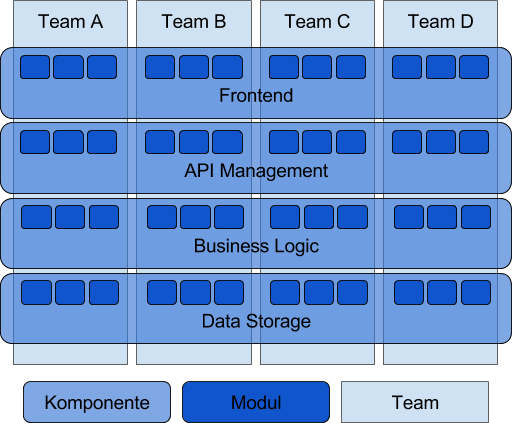
\includegraphics[width=0.40\textwidth]{img/feature-teams.png}} 
    \subfigure[Komponenten-Teams]{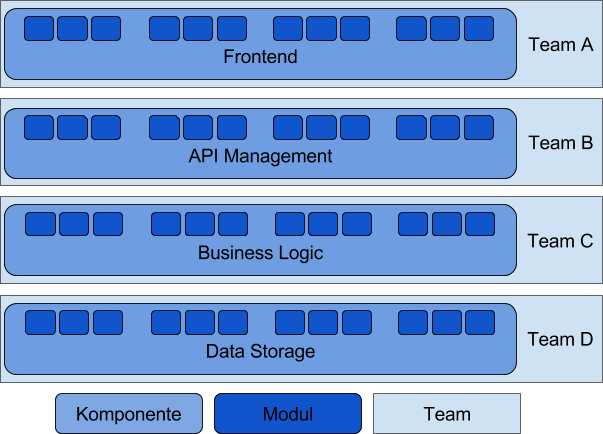
\includegraphics[width=0.48\textwidth]{img/component-teams.png}} 
  \caption{Scrum Teams}\label{fig:Scrum Teams}
  \end{figure}
\end{savenotes}

In allen Varianten existieren aber pro Team unterschiedliche Software-Module und (agile) Prozesse, die unabhängig voneinander die Team-Qualität als gesamtes bestimmen.

\clearpage
\section[Software-Qualität]{Software-Qualität~\footcite[vgl.][Kapitel 1.2]{hoffmann_software_qualitat_2013}}

Eine mögliche Definition von Software-Qualität findet sich in der DIN-ISO-Norm 9126:

\begin{quote}
  Software-Qualität ist die Gesamtheit der Merkmale und Merkmalswerte eines Software-Produkts, die sich auf dessen Eignung beziehen, festgelegte Erfordernisse zu erfüllen.
\end{quote}

Wie aus dieser Definition schon erkennbar ist, gibt es viele unterschiedliche Kriterien, um die Qualität von Software zu bewerten.
Einige wesentliche Merkmale, um die Qualität von Software bewerten zu können, lassen sich in kunden- und herstellerorientierte Merkmale unterteilen:

\begin{description}
  \item[Kundenorientierte Merkmale] \hfill \\ Nach außen hin sichtbare Merkmale, die sich auf den kurzfristigen Erfolg der Software auswirken, da sie die Kaufentscheidung möglicher Kunden beeinflussen.
  \begin{description}
    \item[Funktionalität (Functionality, Capability)] \hfill \\ Beschreibt die Umsetzung der funktionalen Anforderungen. Fehler sind hier häufig Implementierungsfehler (sogenannte Bugs), welche durch Qualitätssicherung bereits in der Entwicklung entdeckt oder vermieden werden können. 
    \item[Laufzeit (Performance)] \hfill \\ Beschreibt die Umsetzung der Laufzeitanforderungen. Besonderes Augenmerk muss in Echtzeitsystemen auf dieses Merkmal gelegt werden.
    \item[Zuverlässigkeit (Reliability)] \hfill \\ Eine hohe Zuverlässigkeit ist in kritischen Bereichen, wie z.B. Medizintechnik oder Luftfahrt, unabdingbar. Erreicht werden kann diese aber nur durch die Optimierung einer Reihe anderer Kriterien.
    \item[Benutzbarkeit (Usability)] \hfill \\ Betrifft alle Eigenschaften eines Systems, die mit der Benutzer-Interkation in Berührung kommen.
  \end{description}
  \item[Herstellerorientierte Merkmale] \hfill \\ Sind die inneren Merkmale, die sich auf den langfristigen Erfolg der Software auswirken und somit als Investition in die Zukunft gesehen werden sollten.
  \begin{description}
    \item[Wartbarkeit (Maintainability)] \hfill \\ Die Fähigkeit auch nach der Inbetriebnahme noch Änderungen an der Software vorzunehmen. Wird oft vernachlässigt, ist aber essentiell für langlebige Software und ein großer Vorteil gegenüber der Konkurrenz.
    \item[Transparenz (Transparency)] \hfill \\ Beschreibt, wie die nach außen hin sichtbare Funktionalität intern umgesetzt wurde. Gerade bei alternder Software, kann es zu einer Unordung kommen, welche auch Software-Entropie (Grad der Unordnung) genannt wird.
    \item[Übertragbarkeit] \hfill \\ Wird auch Portierbarkeit genannt und beschreibt die Eigenschaft einer Software, in andere Umgeungen übertragen werden zu können (z.B. 32-Bit zu 64-Bit oder Desktop zu Mobile).
    \item[Testbarkeit (Testability)] \hfill \\ Testen stellt eine große Herausforderung dar, da oft auf interne Zustände zugegriffen werden muss oder die Komplexität die möglichen Eingangskombinationen vervielfacht. Aber gerade durch Tests können Fehler frühzeitig entdeckt und behoben werden.
  \end{description}
\end{description}

Je nach Anwendungsgebiet und den Anforderungen der Software haben die Merkmale unterschiedliche Relevanz und einige können sich auch gegenseitig beeinflussen, wie aus der Korrelationsmatrix ersichtlich.

\begin{savenotes}
  \begin{figure}[H] 
    \centering
       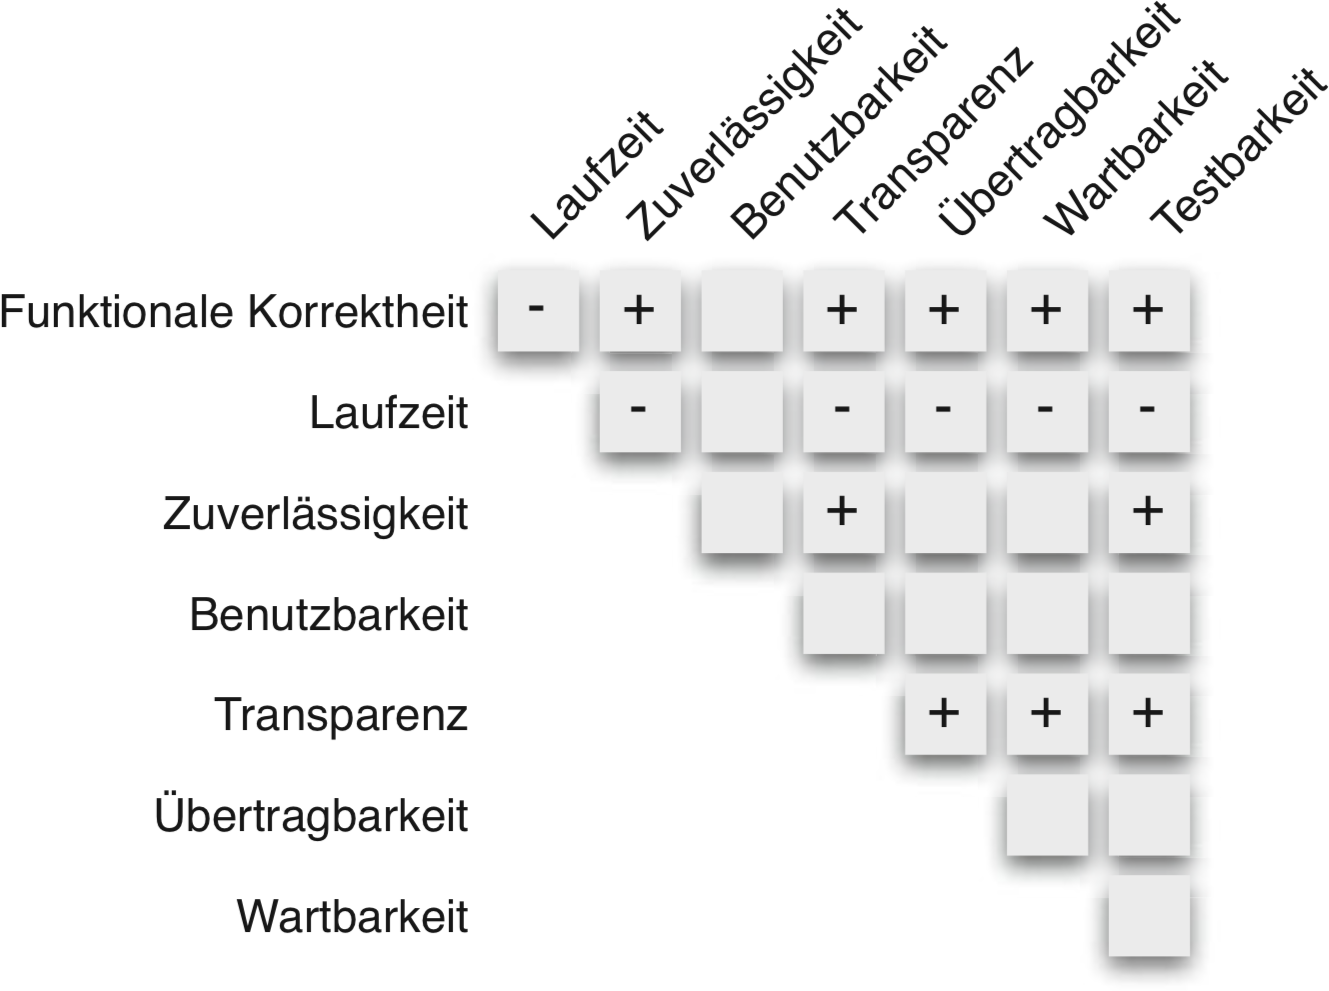
\includegraphics[width=0.6\textwidth]{img/korrelationsmatrix-kriterien.png}
    \caption[Korrelationsmatrix Qualitätskriterien]{Korrelationsmatrix Qualitätskriterien~\footcite[][S. 11, Abb. 1.3]{hoffmann_software_qualitat_2013}}\label{fig:Korrelationsmatrix Qualitätskriterien}
  \end{figure}
\end{savenotes}


\section{Software-Metriken}

Software-Metriken helfen uns dabei, bestimmte (Qualitäts-) Merkmale beziehungsweise Kenngrößen eines Software-Systems systematisch und quantitativ zu erfassen.
Ziel ist es dabei, diese oft versteckten Merkmale sichtbar und vergleichbar zu machen.
Ein einfaches Beispiel ist die \ac{LOC}-Metrik, die die gesamte Anzahl an Zeilen Code darstellt und als grobes Maß für die Komplexität verwendet werden kann.

\subsection{Testmetriken}

\subsection{Softwaremetriken}

\subsection{Agile-Metriken}

\section{Kennzahlen aus dem Entwicklungsprozess}
Einzelne Systeme und ihre Key Metrics / erweiterte Metriken.

\subsection{Versionskontrolle}

\subsection{Continuous Integration}

\subsection{Projektmanagement}

\subsection{Applikationsmonitoring}
